% !TEX root = ../ausarbeitung.tex

\chapter{Entwicklung der Anwendung}

Im Rahmen der Masterarbeit wurde die beschriebende Web Applikation prototypisch entwickelt. Die dazu nötige Planung und die verwendeten Technologien wurden in den vorherigen Kapiteln geschildert. Nun wird auf den Prozess der Entwicklung und auf die detaillierte Struktur der Applikation eingegangen.\\

Das Entwicklung des Systems wurde in drei Teilprojekte untergliedert:
\begin{enumerate}
	\item Erstellung der Basisdatenbank aus dem Wörterbuch CELEX2
	\item Entwicklung des Backends mit python
	\item Entwicklund des Frontends mit gängigen Webtechnologien und AngularDart
\end{enumerate}

Dabei wurde Schritt 1 als Erstes durchgeführt, die Verfügbarkeit der Basisdatenbank war Voraussetzung um mit der Entwicklung von Front- und Backend zu beginnen. Als eine erste Version der Datenbank vorlag, wurde zunächst mit der Entwicklung eines minimalen Backends begonnen, welches die Kernfunktionalität - das Analysieren von Texten - beherrschte. Damit konnte eine erste Version des Frontends erstellt werden, um einen ersten Eindruck zu bekommen, wie alle Technologien miteinander funktionieren.\\
Im Anschluss konnten Front- und Backend parallel entwickelt werden. Es wurden immer wieder Funktionen im Backend entwickelt, woraufhin das Frontend angepasst wurde, um dem Nutzer diese Funktionen anzubieten. Zu diesem Zeitpunkt wurde auch die Basisdatenbank einige male überarbeitet, so ist das Gesamtsystem Schritt für Schritt auf eine agile Weise \tocite{agil} gewachsen. Im Folgenden wird näher auf die drei Teilprojekte eingegangen.

\section{Erstellung einer Basisdatenbank}
\label{sec:worddatabase}

Für die Segmentierung von Wörtern in Silben mit Betonung wird eine sqlite Datenbank verwendet, deren Entwicklung hier beschrieben wird. Als Grundlage für die Datenbank dient das digitale Lexikon \todo{Lexikon/woerterbuch...?} CELEX2, wie in Kapitel \ref{sec:forschung-database} beschrieben. Folgende Informationen wurden dem CELEX entnommen und in der Datenbank gespeichert:

\paragraph{Worttext}
Hier wurde darauf geachtet, eine einheitliche orthographische Form der Wörter durchzusetzen. Wörter bestehen nur aus Kleinbuchstaben (auch die Anfänge von Nomen und Eigennamen). Außerdem wird hier auf Umlaute verzichtet, \qq{ä} wird durch \qq{ae} ersetzt, \qq{ö} durch \qq{oe}, \qq{ü} durch \qq{ue} und \qq{ß} durch \qq{ss}. Beispielsweise wird das Wort \textit{Häuser} zu \textit{haeuser}. So kann beim Nachschlagen garantiert werden, dass ein Wort nicht wegen uneinheitlicher Schreibweise nicht gefunden wird, sofern alle Umlaute vorher ersetzt wurden.

\paragraph{Wortart}
Um Doppeldeutigkeit zu vermeiden wird ein Eintrag nur eindeutig über das Paar aus Worttext und Wortart identifiziert. Viele Grundformen von Verben kommen zum Beispiel auch als Nomen vor, werden aber dann groß geschrieben (\qq{sie sollte die Maschine \textit{verwenden}} gegen \qq{das \textit{Verwenden} der Maschine}). Die Bezeichner für Wortart sind in verschiedenen Systemen wie dem CELEX und dem NLP parser \textit{spacy} unterschiedlich, daher wird hier eine eigene - im Gesamtsystem konsistente - Benennung der Wortart eingeführt (die Benennung orientiert sich an den Tag Namen des spacy parsers, verwendet jedoch zur Unterscheidung Klein- statt Großschreibung):

\begin{table}[h!]
	\centering
	\begin{tabular}{|l|l|}
		\hline
		Wortart & Benennung/Tag \\
		\hline
		\hline
		Nomen & \textit{noun}\\
		Eigenname & \textit{propn}\\
		Verb & \textit{verb}\\
		Hilfsverb & \textit{aux}\\
		Adjektiv & \textit{adj}\\
		Adverb & \textit{adv}\\
		Artikel & \textit{det}\\
		Adposition & \textit{adp}\\
		Pronomen & \textit{propn}\\
		Konjunktion & \textit{conj}\\
		Zahl & \textit{num}\\
		Partikel & \textit{part}\\
		Zahl & \textit{num}\\
		\hline
	\end{tabular}
	\caption{Benennung der Wortarten in der Applikation}
\end{table}

\paragraph{Silbentrennung}
Die Silbentrennung enthält die einzelnen Silben, getrennt durch einen Querstrich (\qq{-}). Im Gegensatz zum Worttext erhält dieser Eintrag Groß- und Kleinschreibung, sowie alle Umlaute. Die Silbentrennung des Wortes \textit{Möglichkeit} ist also \textit{Mög-lich-keit}.

\paragraph{Betonungsmuster}
Das Betonungsmuster identifiziert eine Silbe als Hauptbetonung im Wort. Dieser Eintrag ist ein String aus aneinandergereihten \qq{0} und \qq{1} Werten. Die \qq{1} bezeichnet dabei die betonte Silbe, die \qq{0} stellt eine unbetonte Silbe dar. Nebenbetonungen werden im Rahmen dieser Arbeit vernachlässigt. Das Betonungsmuster besteht nur aus einer einzigen \qq{1} - der Hauptbetonung - während alle anderen Silben unbetont (\qq{0}) bleiben. Beispiel resultiert das Wort \textit{hervorragend} mit der Silbentrennung \textit{her-vor-ra-gend} in das Betonungsmuster \qq{0100}.

\paragraph{Lemma}
\todo{was genau? auch im celex, keine wirkliche anwendung in der app, vielleicht ausblick}

Neben den Worteinträgen sollen in der Datenbank noch Informationen über die Herkunft der Wörter gespeichert werden. Neben den Basiseinträgen, die aus dem CELEX extrahiert werden, wird den Nutzern später die Möglichkeit gegeben Einträge zur Datenbank hinzuzufügen. Um diesen Vorgang nachvollziehbar zu machen gibt es eine zweite Tabelle, in welcher Einträge für neu hinzugefügte Wörter mit Zeitstempel angelegt werden. Das Folgende Schema \ref{fig:worddatabase} zeigt die Struktur der Wortdatenbank.

\begin{figure}[h!]
	\centering
	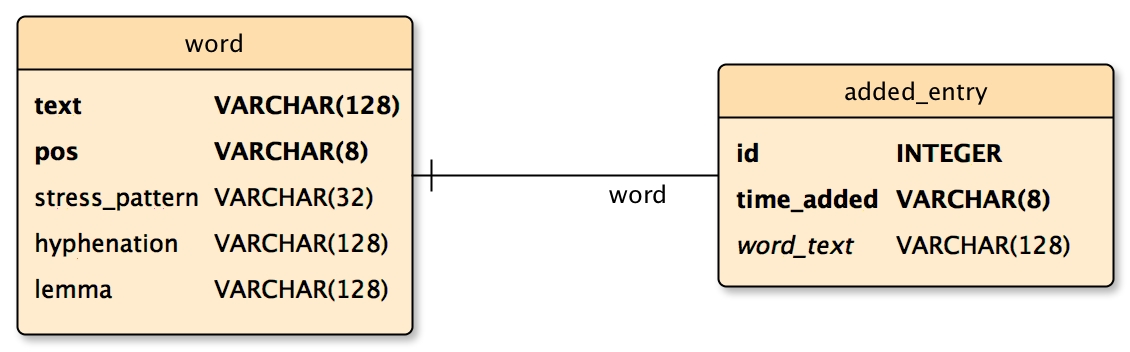
\includegraphics[width=.6\linewidth]{figures/worddb}
	\caption{Schema der Wortdatenbank (\textit{word.db})}
	\label{fig:worddatabase}
\end{figure}

Alle in der Worttabelle beschriebenen Einträge sind auch im CELEX vorhanden. Der Folgende Abschnitt beschreibt, wie die Daten aus dem Lexikon extrahiert und in der Wortdatenbank gespeichert wurden.

\subsection{Implementierung}

Für die Generierung der Datenbank wurde das python Projekt \textit{celex2db} erstellt, welches in \qq{/backend/celex2db} zu finden ist (alle Pfadangaben in diesem Abschnitt beziehen sich auf dieses Verzeichnis). Die Daten im CELEX \todo{in Forschungsstand teil verschieben} sind über mehrere Dateien verteilt. So gibt es eine Teilung in Sprachen (für die Datenbank werden nur Deutsche Wörter benutzt, zu finden in \qq{celex2/german}), Wörter und Lemmata sowie in Orthographie, Phonologie und Morphologie. Die Teilung in Wort und Lemma spart Speicherplatz. Das Lemma eines Verbs, zum Beispiel, ist die Grundform dieses. Zur Beugung \textit{gehst} gehört also das Lemma \textit{gehen}. Viele Eigenschaften des Verbs \textit{gehen} beziehen sich auf alle Flexionsformen, so müssen diese nicht für alle Verbformen redundant gespeichert werden.\\
Die Einträge in den Wortlisten des CELEX verweisen jeweils mit einer ID auf den zugehörigen Eintrag in der Lemma Liste. Da in der zu entwickelnden Datenbank auch das Lemma gespeichert werden soll, müssen sowohl Wort Listen als auch Lemma Listen geparsed werden.\\

Das Hauptskript \qq{celex2db.py} führt die folgenden Schritte aus:
\begin{enumerate}
	\item Parsen der orthographischen Lemma Liste
	\item Parsen der orthographischen und phonologischen Wort Listen
	\item Generierung von Einträgen aus Wort und Lemma Listen und Schreiben in die Datenbank
\end{enumerate}
Während der Ausführung des Skripts werden Schrittweise Fortschrittsangaben mit Fehlern ausgegeben (Schrittweite im Skript einstellbar), da das Parsen und Erstellen der Datenbank einige Zeit benötigt (mehr dazu im Abschnitt \ref{sec:database-results}).

Die Klasse \texttt{CelexDictionary} im Skript \qq{celex.py} bietet die Methoden zum Parsen der Wort und Lemma Listen. Die Struktur ist in \ref{fig:celex2db} dargestellt.\\

\begin{figure}
	\centering
	\todo{Klassendiagramm CelexDictionary}
	\caption{Diagramm der \textit{celex2db} Klassen}
	\label{fig:celex2db}
\end{figure}

In der \texttt{parseLemma} Methode wird die CELEX Datei \qq{gml.cd} verarbeitet. Die morphologische Informationen zu den Lemmata enthält. Jede Zeile enthält ein Lemma, für welches in der Struktur \texttt{CelexLemma} die ID des Lemmas, Text und Wortart gespeichert werden.\\

In der \texttt{parseWords} Methode werden nun die beiden Dateien \qq{g\textbf{p}w.cd} und \qq{g\textbf{o}w.cd} verarbeitet, welche phonologische und orthographische Informationen zu allen enthaltenen Beugungen der Wörter enthalten. Die IDs und Reihenfolge in beiden Wortlisten stimmen überein, sodass beide Listen gleichzeitig verarbeitet werden können. Aus der phonologischen Liste werden der Text des Wortes, der Verweis auf das zugehörige Lemma (lemma\_id) sowie die phonologische Darstellung entnommen. Die orthographischen Liste liefert lediglich die Silbentrennung.\\
Danach wird in der zuvor verarbeiteten Liste der Lemmas, mithilfe der \texttt{lemma\_id} der Text passende Lemmas gesucht und alle verfügbaren Daten in der Struktur \texttt{CelexWord} gespeichert. Die Hauptklasse \texttt{CelexDictionary} enthält ein python Dictionary aller \texttt{CelexWord} Einträge, siehe Abbildung \ref{fig:celex2db}.

Letztendlich werden die Einträge der Wortliste im Skript \qq{writeSQLite.py} in die Datenbank übertragen. In einem frühen Entwicklungsstadium wurden hier SQL Instruktionen verwendet um die Datenbankeinträge zu erstellen. Nach der Entwicklung des \texttt{DictionaryService} im Backend (genauer beschrieben im Abschnitt \ref{sec:dictionary-service}wurde später direkt auf diesen zugegriffen, um Redundanten Code zu vermeiden. Ein einfacher Funktionsaufruf der Methode \texttt{add\_word} des \texttt{DictionaryService} fügt den Eintrag der Wortdatenbank hinzu.

\subsection{Ergebnisse}
\label{sec:database-results}

Ein Wort soll eindeutig identifizierbar sein durch den Worttext und die Wortart. Daher wurde in der Datenbank die Kombination der Felder \textit{text} und \textit{pos} (part of speech/Wortart) als Primärschlüssel gewählt. Ein doppeltes Einfügen eines Wortes in die Datenbank verletzt den SQL \textit{UNIQUE Constraint}, und ist somit nicht möglich. Die dadurch von python geworfene Exception wird in diesem Fall abgefangen und und die \texttt{add\_word} Methode liefert \texttt{None} zurück.\\
Trotz der Wortidentifizierung anhand von zwei Merkmalen, beinhaltet der CELEX teilweise redundante Informationen. 4 356 Einträge verursachen aufgrund des \textit{UNIQUE Constraint} Fehler, da sie mit gleichem Text und gleicher Wortart schon in der Datenbank waren, diese wurden somit übersprungen. Bei einem kompletten Neuaufbau der Datenbank aus dem CELEX werden 360 243 Wörter hinzugefügt. Die Datenbank wurde als sqlite Datei \qq{/backend/db/words.db} angelegt.

\section{Backend}
\label{sec:etwicklung-backend}
Das in python mit dem Web-Framework flask entwickelte Backend verarbeitet sämtliche, vom Frontend gesendeten HTTP requests. Es sendet entweder eine Antwort mit den geforderten Daten oder einen HTTP Fehlercode mit Fehlermeldung. Das Backend Projekt befindet sich in \qq{/backend/API}. Es wurde in die drei Services \textit{DictionaryService}, \textit{UserService} und \textit{VerificationService} strukturiert. Das Hauptsript \todo{rename} \qq{LinguisticTextAnnotation.py} verwaltet diese Services, startet die flask Applikation und definiert die einzelnen Routen für HTTP requests (diese werden im folgenden Abschnitt aufgelistet). Folgende Grafik zeigt eine Übersicht über die Struktur des Backends.

\todo{Grafik Backend}

\subsection{HTTP Routen}
Tabelle \ref{table:backendroutes} bietet eine Übersicht über die verfügbaren Routen, welche die HTTP requests verarbeiten. Zudem werden kurz der Zweck und die Parameter der Route beschrieben. Ein \textit{X} in der Spalte Authentifizierung bedeutet, dass die Mail Adresse und das Passwort des Nutzers übergeben werden muss. Diese werden nicht extra in der Spalte Parameter aufgeführt (außer in der \qq{/user/authenticate} Route, diese dient ausschließlich dazu, die Übermittelten Nutzer Credentials zu prüfen).

\begin{table}[h!]
	\centering
	\begin{tabular}{|l|l|l|c|}
		\hline
		\textbf{Route} & \textbf{Parameter} & \textbf{Methode} & \textbf{Auth.}\\
		\hline
		\hline
		/query/word & text, pos & GET & \\
		\hline
		/query/text & text & POST & \\
		\hline
		/query/segmentation& word & GET & \\
		\hline
		\hline
		/user/register & email, password, & POST & \\
		& first\_name, last\_name, is\_expert &&\\
		\hline
		/user/authenticate & \textit{email, password} & POST & X\\
		\hline
		/user/delete & id & POST & X\\
		\hline
		\hline
		/user/word/add& text, stress\_pattern, hyphenation, pos & POST & X\\
		\hline
		/user/word/delete& id & POST & X\\
		\hline
		/user/word/list & - & POST & X\\
		\hline
		\hline
		/user/configuration/add & name, \textit{options} & POST & X\\
		\hline
		/user/configuration/update & id, name, \textit{options}  & POST & X\\
		\hline
		/user/configuration/list & - & POST & X\\
		\hline
		/user/configuration/delete & id & POST & X\\
		\hline
		\hline
		/user/text/add & title, text & POST & X\\
		\hline
		/user/text/delete & id & POST & X\\
		\hline
		/user/text/list & - & POST & X\\
		\hline
		\hline
		/user/verification/query & - & POST & X\\
		\hline
		/user/verification/submit & id, stress\_pattern, hyphenation & POST & X\\
		\hline
	\end{tabular}
	\caption{Backend routen für HTTP requests mit Parametern und Methode}
	\label{table:backendroutes}
\end{table}

Die bei \qq{user/configuration/} nicht aufgeführten \textit{options} bestehen aus allen für die Annotationsvorlage gespeicherten einstellungen. Dies sind die Folgenden Felder: \textit{stressed\_color, unstressed\_color, word\_background, alternate\_color, syllable\_separator, line\_height, word\_distance, syllable\_distance, font\_size, letter\_spacing, use\_background, highlight\_foreground, stressed\_bold, use\_alternate\_color, use\_syllable\_separator, part\_of\_speech\_configuration}.

\subsection{Dictionary Service}
\label{sec:dictionary-service}

Das Modul \textit{DictionaryService.py} verarbeitet Anfragen zur Textanalyse, verwaltet die Wortdatenbank und generiert Vorschläge für die manuelle Segmentierung von Wörtern. Das Schema der Wortdatenbank zeigt Abbildung \ref{fig:worddatabase}. Folgende Klassen werden definiert:
\begin{itemize}
	\item \texttt{Word}: Entspricht Tabelle \textit{word} in der Wortdatenbank (Abbildung \ref{fig:worddatabase}) und speichert die Merkmale eines Wortes.
	\item \texttt{AddedEntry}: Enthält einen Verweis (Fremdschlüssel) auf ein hinzugefügtes Wort und dessen Erstellungszeitpunkt.
	\item \texttt{Segmentation}: Modelliert einen Segmentierungsvorschlag. Die Klasse enthält Worttext, Segmentierung und Betonungsmuster. Außerdem speichert sie den Namen (\texttt{origin}) und die Herkunft (\texttt{source}) der Quelle des Vorschlags (z.B. MARY TTS).
\end{itemize}

Im Folgenden werden die Funktionen des \textit{DictionaryService} genauer beschrieben.

\subsubsection{Funktionen der Wortdatenbank}
\begin{itemize}
	\item Die Methode \texttt{add\_word} bekommt Worttext, Betonungsmuster, Wortteilung, Lemma und Wortart übergeben (s. Abschnitt \ref{sec:worddatabase}), fügt das Wort der Datenbank hinzu und liefert eine \texttt{Word} Instanz zurück. Im Falle eines Fehlers oder falls das Wort schon existiert, gibt die Methode \texttt{None} zurück.
	
	\item \texttt{query\_word} schlägt ein Wort mit den Parametern Worttext und Wortart in der Datenbank nach und gibt das annotierte Wort im JSON (\textit{text}, \textit{stress\_pattern}, \textit{hyphenation}, \textit{lemma}, \textit{pos}) Format zurück. Als Parameter kann optional der eingeloggte Nutzer übergeben werden. Ist das der Fall, wird zuerst überprüft, ob im Nutzeraccount (s. Abschnitt \ref{sec:userservice}) eine manuelle Segmentierung für das Wort gespeichert ist und falls ja, diese zurückgegeben. Werden in der Wortdatenbank mehrere Wörter gefunden, die dem gesuchten Worttext entsprechen, wird zusätzlich die Wortart geprüft und der passende Eintrag (bzw. der Erste Eintrag, falls kein Wort mit der entsprechenden Wortart gefunden wird) zurückgegeben.
	
\subsubsection{Textanalyse}
Die Methode \texttt{query\_text} bekommt den gesamten zu analysierenden Text übergeben (sowie optional den eingeloggten Nutzer für manuelle Worteinträge). Der Text wird zunächst mit dem spacy Parser analysiert. Dieser zerlegt den Text in einzelne Wörter und Trennzeichen und gibt eine Liste von Tokens zurück. Nun wird über die Liste der Tokens iteriert und dabei wiederum eine Liste von JSON Einträgen generiert, welche am Schluss von der Methode zurückgegeben wird. Jedes spacy Token liefert den Worttext \texttt{text} die Wortart \texttt{pos\_} und das Lemma \texttt{lemma\_}. Das Token wird wie folgt verarbeitet:

\begin{enumerate}
	\item In jedem Fall wird ein neuer JSON Eintrag angelegt und die Felder \texttt{text}, \texttt{pos} und \texttt{lemma} mit den entsprechenden Inhalt des spacy Tokens gefüllt.
	
	\item Enthält der Worttext einen Linebreak \qq{\texttt{\textbackslash n}}, so wird das JSON Feld \texttt{type} mit \textit{linebreak} belegt.
	
	\item Enthält der Worttext einen Trennstrich \qq{\texttt{-}}, so handelt es sich um ein zusammengesetztes Wort (z.B. \textit{100-Millionen-Einwohner-Staat}). Hier werden alle Trennstriche durch Leerzeichen ersetzt. Der resultierende String wird dann erneut mit spacy analysiert und die Tokens dann entsprechend verarbeitet. Hinter jedem Teilwort (außer dem Letzten) wird manuell der Trennstrich als eigenes Token eingefügt.
	
	\item Entspricht der Wortart-Tag einem String aus \texttt{['X',} \texttt{'PUNCT', }\texttt{'NUM', }\\
	\texttt{'SPACE']}, so handelt es sich um eine dem Parser unbekannte Zeichenfolge, eine Zahl, ein Satz- oder Leerzeichen. Diese Tags werden nicht nachgeschlagen sondern mit dem JSON \texttt{type} Feld \textit{ignored} der Rückgabeliste hinzugefügt.
	
	\item Trifft keiner dieser Sonderfälle zu, wird das Wort mit der Methode \texttt{query\_word} nachgeschlagen. Wird dieses gefunden (Rückgabewert nicht \texttt{None}), wird der \texttt{type} auf \textit{annotated\_word} gesetzt. Das JSON Feld \texttt{annotation} enthält dann die Informationen des annotierten Wortes (von \texttt{query\_word} zurückgegeben). Ist das Wort nicht in der Datenbank, so enthält das Feld \texttt{type} den Wert \textit{not\_found}.
\end{enumerate}

\end{itemize}

\subsubsection{Generierung von Segmentierungsvorschlägen}
\label{sec:segmentation-proposals}

Der \texttt{DictionaryService} bietet auch die Möglichkeit, automatisch Segmentierungsvorschläge zu generieren. Diese werden im Frontend dazu benutzt, den NutzerInnen bei der manuellen Wortsegmentierung die Arbeit zu erleichtern, indem das Wort schon in Silben zerlegt wird und versucht wird, automatisch die Wortbetonung zu bestimmen. Der Standardvorschlag, den das System liefert ist einfach die Silbentrennung, die der Python Silbentrenner \textit{Pyphen} liefert. Diese ist in vielen Fällen korrekt und bietet in jedm Fall einen Anhaltspunkt für die Silbentrennung des Wortes. Zudem wird beim Standardvorschlag ein Betonungsmuster generiert, welches immer die erste Silbe im Wort betont. Auch das ist in der Deutschen Sprache oft der Fall, so können Betonung und Silbentrennung bei der manuellen Analyse einfach bestätigt werden.\\

Bei der Abfrage der Vorschläge im Backend wird eine Liste von Segmentierungsvorschlägen zurückgeliefert. Der Standardvorschlag mit \textit{Pyphen} ist nur eine Möglichkeit. Hier wurde überlegt, aus mehreren externen Systemen, wie z.B. MARY TTS oder BAS (s. Abschnitt \ref{sec:forschung-database}), oder später auch z.B. Duden und Anderen, Vorschläge zu sammeln und den NutzerInnen in einer Liste zu präsentieren, aus der der passendste Vorschlag ausgewählt werden kann. Exemplarisch wurde hier eine Anfrage an MARY TTS geschickt und in der Antwort an das Frontend mit eingebunden. Das System kann ebenfalls mit HTTP Requests abgefragt werden. Das entsprechende Interface ist unter \textit{http://mary.dfki.de:59125/process} zu finden. Tabelle \ref{table:mary} zeigt die bei der Anfrage verwendeten GET Parameter. MARY liefert eine Antwort im XML Format zurück, die die phonologische Silbentrennung und die Betonung enthält. Das XML wird entsprechend geparsed, womit dann ein neuer Segmentierungsvorschlag bestimmt werden kann.

\begin{table}[h!]
	\centering
	\begin{tabular}{|l|l|}
		\hline
		\textbf{Parameter} & \textbf{Wert}\\
		\hline
		\hline
		INPUT\_TEXT & \textit{das abzufragende Wort}\\
		INPUT\_TYPE & TEXT\\
		OUTPUT\_TYPE & ACOUSTPARAMS\\
		LOCALE & de\\
		\hline
	\end{tabular}
	\caption{GET Parameter für Anfrage an MARY TTS}
	\label{table:mary}
\end{table}

\subsection{User Service}
\label{sec:userservice}

Der \texttt{UserService} dient der Verwaltung der Nutzerdaten und der Authentifizierung. Nutzerkonten bestehen aus Email Adresse, Passwort und Vor- und Nachnamen der Nutzerin oder des Nutzers. Daneben werden die Resourcen \textit{user\_text}, \textit{user\_word}, \textit{text\_config} und \textit{pos\_config} verwaltet. Welche Funktionen für die jeweilige Ressource zur Verfügung stehen, wird im Folgenden erklärt. Abbildung \ref{fig:userdb} zeigt das Schema der Nutzerdatenbank.

\begin{figure}[h!]
	\centering
	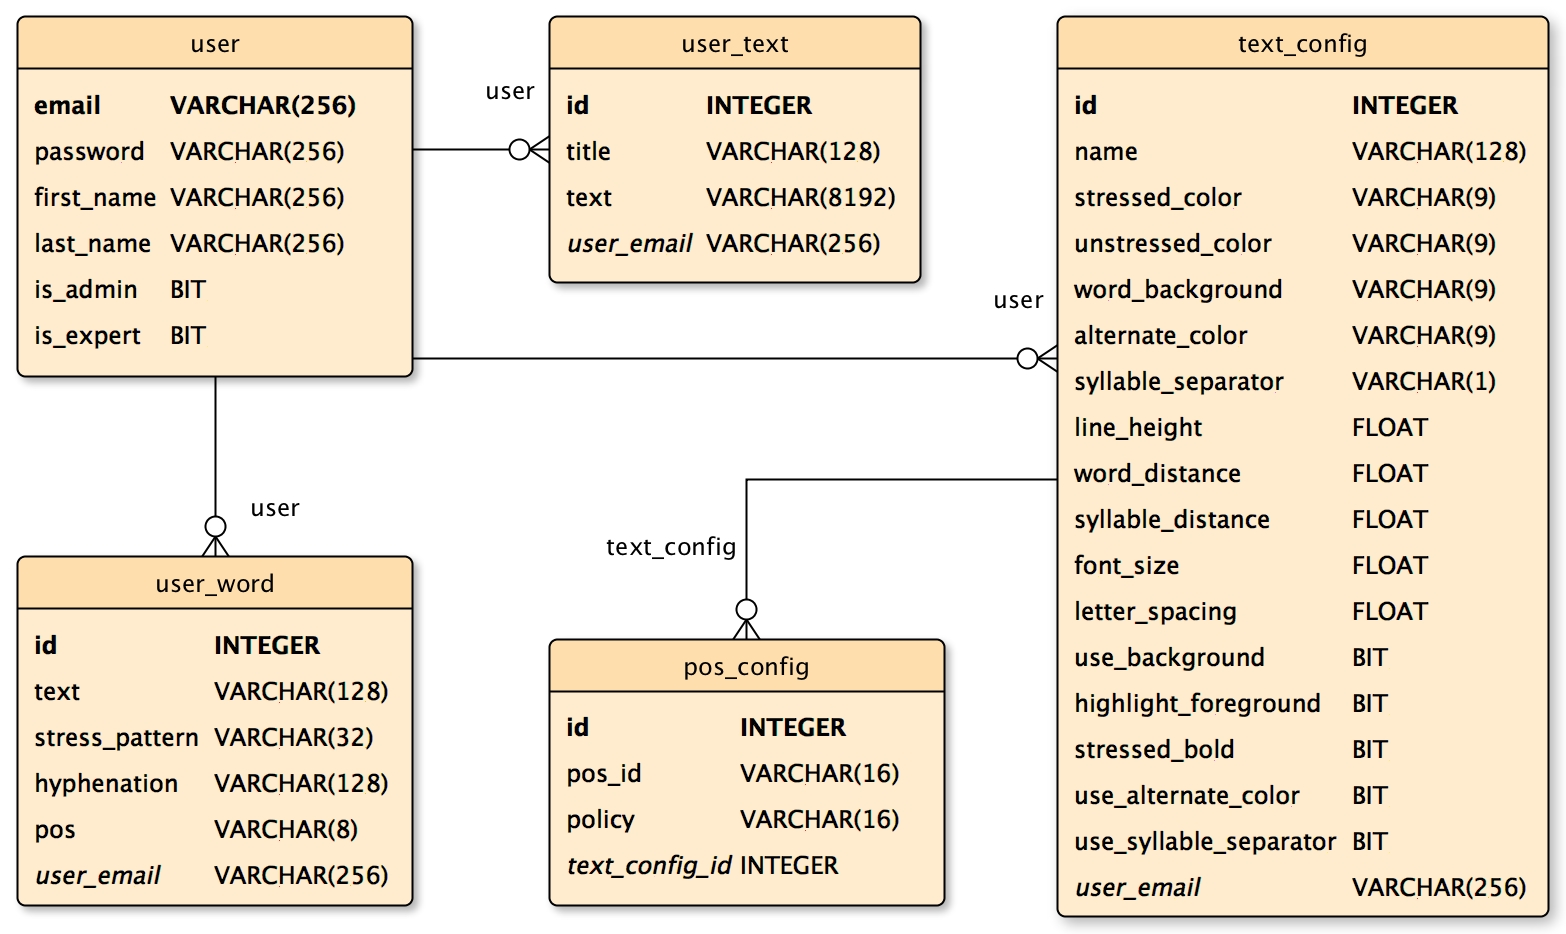
\includegraphics[width=.8\linewidth]{figures/userservicedb}
	\caption{Schema der User Datenbank (\textit{user.db})}
	\label{fig:userdb}
\end{figure}

\begin{itemize}
	\item Zur \textbf{Authentifizierung} wird überprüft, ob ein Nutzerkonto für die als Parameter übergebene Email Adresse und das übermittelte Passwort existiert.
	
	\item \textbf{Nutzertexte} (\textit{user\_text}) können mit Text und Titel erstellt, sowie mit entsprechenden Anfragen abgefragt (als Liste aller Texte eines Nutzerkontos) oder entfernt werden.
	
	\item Auch für \textbf{Nutzerwörter} (\textit{user\_word}, Einträge, die durch die manuelle Segmentierung entstehen), können mit Text, Silbentrennung, Betonungsmuster und optional Wortart angelegt, sowie abgefragt (ebenfalls als Liste aller Wörter eines Nutzerkontos) oder gelöscht werden.
	
	\item Für \textbf{Annotationskonfigurationen} (\textit{text\_config}) gibt es vier Funktionen: Sie können als Liste abgefragt oder mit der zugehörigen \textit{id} gelöscht werden, sowie angelegt und aktualisiert werden. Beim Anlegen und Aktualisieren werden sämtliche Attribute der Konfiguration (Name, Silbenfarben, Texteinstellungen, wie Silben- oder Wortabstand etc.) in der Anfrage mit übergeben. Auch die Konfigurationsliste für die Wortarten (\textit{pos\_config}), die für jede Wortart die Einstellung, ob diese annotiert oder ignoriert wird speichert, wird in der Anfrage benötigt.
\end{itemize}


\subsection{Verification Service}
\label{sec:verification-service}

Von den NutzerInnen manuell erstellte Segmentierungen für Wörter können nicht direkt in die globale Wortdatenbank für alle Nutzer übernommen werden, da bei der Segmentierung Fehler gemacht werden können. Der \texttt{VerificationService} definiert die Funktionen mit denen zu verifizierende Segmentierungen abgefragt oder Verifizierungsvorschläge abgeschickt werden können.\\
Ein zu verifizierender Eintrag ist hierbei direkt ein \textit{user\_word} (s. Abbildung \ref{fig:userdb}), dass von einer Nutzerin oder einem Nutzer bei der manuellen Segmentierung erstellt wurde. Die Verifizierung (Klasse \texttt{VerificationProposal}) bezieht sich auf diesen Eintrag und enthält ebenfalls Silbentrennung und Betonungsmuster für das Wort. Nach der Übermittlung eines Verifizierungsvorschlags prüft ein Algorithmus, ob ausreichend Verifizierungen unterschiedlicher NutzerInnen für das Wort übereinstimmen (also Silbentrennung und Betonung identisch sind). Ist dies der Fall, wird das Wort in die globale Wortdatenbank übernommen und alle Verifizierungsvorschläge werden wieder entfernt. Im Folgenden wird der Verifizierungsalgorithmus (dieser wird dann verwendet, wenn ein neuer Verifizierungsvorschlag übermittelt wird) kurz vorgestellt:

\begin{enumerate}
	\item Für den übermittelten Vorschlag wird ein \texttt{VerificationProposal} Objekt in der Nutzerdatenbank angelegt.
	
	\item Der Vorschlag erhält initial den \texttt{score} $0$. Es wird über alle Vorschläge, die sich auf das Wort beziehen iteriert, dabei werden Silbentrennung und Betonungsmuster verglichen. Bei Übereinstimmung wird der \texttt{score} erhöht, die Gewichtung ergibt sich je nachdem, ob der Autor des Vorschlags ein normaler Nutzer, Experte oder Administrator ist. Vorschläge von Administratoren erhalten drei, Expertenvorschläge zwei Punkte und normale NutzerInnen einen Punkt.
	
	\item Wird die Zielwertung von $3$ nicht erreicht, so wird abgebrochen. Bei der Übermittlung des nächsten Vorschlags kann so wieder überprüft werden, ob genug Verifizierungen einstimmig sind.
	
	\item Bei einem Score von $3$ kann wird das Wort in die globale Wortdatenbank übertragen. Bei der gegebenen Punkteverteilung geschieht das, sobald entweder ein Administrator, ein Experte und mindestens ein anderer, beliebiger Nutzer, oder drei normale NutzerInnen identische Vorschläge übermitteln.
	
	\item Sowohl, die manuelle Segmentierung für das Wort, sowie alle Verifizierungsvorschläge werden nun nicht mehr gebraucht und daher aus der Datenbank gelöscht.
	
	\item Zudem wird ein Eintrag \texttt{AddedEntry} angelegt, der einen Verweis auf das verifizierte, neue Wort in der Wortdatenbank enthält und einen Zeitstempel mit dem Erstellungszeitpunkt. So kann nachvollzogen werden, welche Wörter wann durch den Verifizierungsprozess der Datenbank hinzugefügt wurden.
\end{enumerate}

\todo{datenbank schema}\\










\section{Frontend}

Das Frontend ist der den Nutzerinnen und Nutzern sichtbare Teil des Softwaresystems. Die Web-Applikation ist zunächst wie eine normale Webseite aufgebaut, Inhalte der Komponenten werden aber dynamisch geladen (d.h. bei Nutzerinteraktionen wird keine Seite neu aufgerufen, sondern der Inhalt der Seite wird direkt angepasst). Neben den standardmäßig im Web verwendeten Sprachen \textit{HTML}, \textit{CSS} und \textit{JavaScript} wurde die Applikation großteils in AngularDart entwickelt (eine genauere Beschreibung zu dieser Technologie, der Unterteilung von Komponenten in Klassen, Templates und Services sowie der Templatesprache von Angular, liefert Abschnitt \ref{sec:angulardart}).\\

Die kombinierten Features von \textit{Angular} und der Programmiersprache \textit{Dart} ermöglichen eine strukturierte objektorientierte Architektur der Applikation. Die Folgenden Abschnitte zeigen zunächst den Aufbau der Applikation und das verwendete Datenmodell, danach die Struktur aller größeren Komponenten.

\subsection{Hauptkomponente der Applikation und Routing}

Die Hauptseite \qq{index.html} enthält nur einen Platzhalter (Kasten mit dem Text \qq{Prosodiya Online Text Analyse wird geladen...}) und bindet notwendige CSS Styles sowie die Hauptkomponente \textit{AppComponent} ein. Das Einbinden dieser Komponente veranlasst Angular, diese beim Aufruf der Webseite zu laden und liefert so den Einstiegspunkt in die \textit{AngularDart} Applikation.\\

Der zur Komponente zugehörige Service \texttt{app\_service} definiert lediglich die Funktionen zum Setzen und Löschen von Info- und Fehlermeldungen. Das Template der Hauptkomponente \qq{app\_component.html} enthält folgende Elemente:
\begin{itemize}
	\item Die Navigationsleiste mit den Einträgen \textit{Home}, \textit{Textanalyse}, \textit{Verifizierung} und \textit{Login.}
	
	\item Container in denen Info- und Fehlermeldungen angezeigt erden
	\item Die \texttt{router-outlet} Direktive, die dafür sorgt, dass die in der Navigation ausgewählte Komponente angezeigt wird
\end{itemize}

In der Komponentenklasse \texttt{AppComponent} werden folgende Metadaten der Applikation per Klassenannotationen definiert:
\begin{itemize}
	\item \textbf{Angular Direktiven} in \textit{@Component}: Alle Basiskomponenten (\texttt{CORE\_DIRECTIVES}, \texttt{ROUTER\_DIRECTIVES}, \texttt{materialDirectives},
	\texttt{formDirectives}) und eigene Subkomponenten (\texttt{TextAnalysisComponent}, \texttt{UserAccountComponent},\\
	\texttt{WordReviewComponent}, \texttt{WordVerificationComponent}, \texttt{HomeComponent},\\
	\texttt{UserRegisterComponent}) werden hier eingebunden und können damit in allen Templates verwendet werden \todo{stack: directives, einbinden erklären}
	
	\item \textbf{Angular Providers} in \textit{@Component}: Alle vordefinierten (\texttt{ROUTER\_PROVIDERS},\\ \texttt{materialProviders}) und eigenen Provider (\texttt{TextAnalysisService},\\
	\texttt{UserAccountService}, \texttt{AppService}, \texttt{SegmentationProposalService},\\ \texttt{SegmentationVerificationService}) werden hier der Applikation bekannt gemacht, sodass sie von allen Komponenten verwendet werden können
	
	\item \textbf{Routen} für den Angular Router werden in \textit{@RouteConfig} zu den entsprechenden Komponenten zugeordnet (s. Tabelle \ref{table:routeconfig})
\end{itemize}

\begin{table}
	\centering
	\begin{tabular}{|l|l|l|}
		\hline
		\textbf{Route} & \textbf{Name} & \textbf{Komponente}\\
		\hline
		\hline
		/\textit{home} & \textit{Home} & \textit{HomeComponent} \\
		\hline
		/text\_analysis & TextAnalysis & TextAnalysisComponent \\
		\hline
		/text\_analysis/:text & TextAnalysisParam & TextAnalysisComponent \\
		\hline
		/word\_review/:wordIndex & WordReview & WordReviewComponent \\
		\hline
		/word\_verification & WordVerification & WordVerificationComponent \\
		\hline
		/user\_account & UserAccount & UserAccountComponent \\
		\hline
		/user\_register & UserRegister & UserRegisterComponent \\
		\hline
		/** & NotFound & HomeComponent \\
		\hline
	\end{tabular}
	\caption{Routen für den Angular Router, mit Name und zugehöriger Komponente. Die kursiv dargestellte \textit{Home} Route ist der Default Wert und wird bei Programmstart angezeigt}
	\label{table:routeconfig}
\end{table}

\subsubsection{Begrüßungsseite}

\begin{figure}[h!]
	\centering
	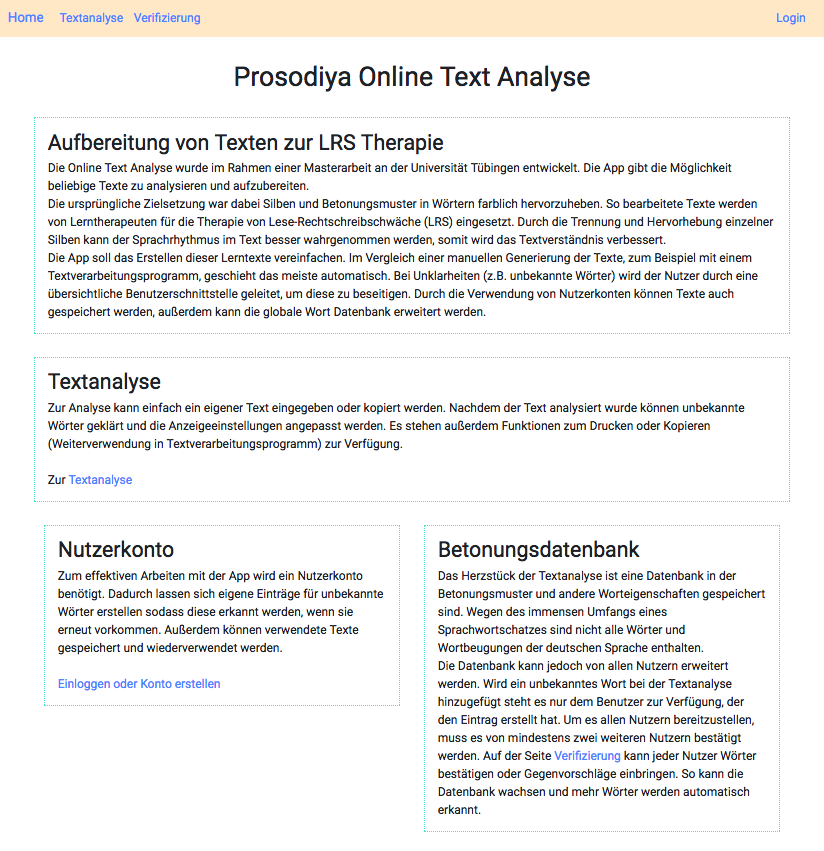
\includegraphics[width=.6\linewidth, frame]{figures/frontend/home}
	\caption{Bildschirmfoto der Begrüßungsseite}
	\label{fig:frontend-home}
\end{figure}

Die Begrüßungsseite (Abbildung \ref{fig:frontend-home}) \textit{home\_component} beinhaltet keine Programmlogik. Sie ist der Einstiegspunkt der Web-Applikation und stellt eine Übersicht über die gebotenen Funktionen dar. In den oberen zwei Kästen findet die Nutzerin oder der Nutzer eine kurze Einführung in die Software und ihre Anwendung, sowie eine Erklärung der Textanalyse Funktion. Darunter befinden sich nebeneinander zwei Kästen, in denen die Nutzerkontoverwaltung und der Verifizierungsprozess für die Wortdatenbank erklärt werden.

\subsection{Datenmodell}

Im Folgenden wird ein Überblick über das Datenmodell gegeben, dessen Klassen diverse Komponenten der Applikation benutzen. Die Klasse \texttt{AnnotationText} wird instantiiert wenn ein neuer Text analysiert wird. Sie
enthält eine Liste von Wörtern (Klasse \texttt{Word}), welche wiederum eine Liste von Silben (Klasse \texttt{Syllable}) speichern. \\

\todo{Klassendiagramm AnnotationText, Word, Syllable}

Diese Klassen enthalten auch Informationen zu HTML Klassen und CSS Styles. Durch entsprechende Zugriffe können diese dann direkt im Angular HTML Template ausgelesen werden. Mit dieser Vorgehensweise ist es möglich, die Textvorschau direkt und verzögerungsfrei nach einer Nutzereingabe anzupassen. Wird zum Beispiel eine Silbenfarbe geändert wird erst über alle Wörter und Silben im \texttt{AnnotationText} iteriert und die entsprechenden CSS Farben (z.B. \texttt{color} oder \texttt{background-color}) auf die neue Farbe gesetzt. Der Angular Update Cycle \todo{heisst das so?} detektiert die Veränderung im Modell und passt das Document Object Model (DOM) der Webseite automatisch an. Es musste kein manueller Code geschrieben, durch \textit{Data Binding} werden die aktuellen Werte im Modell (Dart Klassen) sofort automatisch in das DOM übernommen.\\

Zur Verwaltung von Vorlagen zur Einstellung der Annotation wird die Klasse \texttt{TextConfiguration} verwendet. Sie enthält alle Einstellungen, die auf einen Text angewandt werden können, z.B. die Farben von betonter und unbetonter Silben, Silben- und Wortabstände oder das Silbentrennzeichen. Außerdem beinhaltet sie eine Instanz der Klasse \texttt{PartOfSpeech}, welche spezielle Annotationseinstellungen für die verschiedenen Wortarten speichert.
\todo{Klassendiagramm TextConfiguration und PartOfSpeech}\\

Die Klasse \texttt{UserEntry} bildet die manuell segmentierten Wörter ab, die dem System unbekannt waren und vom Nutzer selbst erstellt wurden. Ein \texttt{UserEntry} enthält Informationen über Worttext, Wortart, Segmentierung der Silben und Wortbetonung. Vom Nutzer angelegte, eigene Texte werden in der Klasse \texttt{UserText} (mit dem Wortlaut des Texts und einem Titel) abgebildet.
\todo{Klassendiagramm von UserEntry und UserText}

\subsection{Textanalyse}

Die Text Analyse stellt das Herzstück der Applikation dar und ist in der Komponente \textit{text\_analysis\_component} abgebildet. Sie bindet mehrere Subkomponenten ein, die in den folgenden Abschnitten vorgestellt werden. Es gibt Nutzeroberflächen für
\begin{itemize}
	\item die Eingabe neuer Texte,
	\item die Vorschau des aktuell analysierten Texts,
	\item sowie die Manuelle Analyse dem System unbekannter Wörter.
\end{itemize}

\begin{figure}[h!]
	\centering
	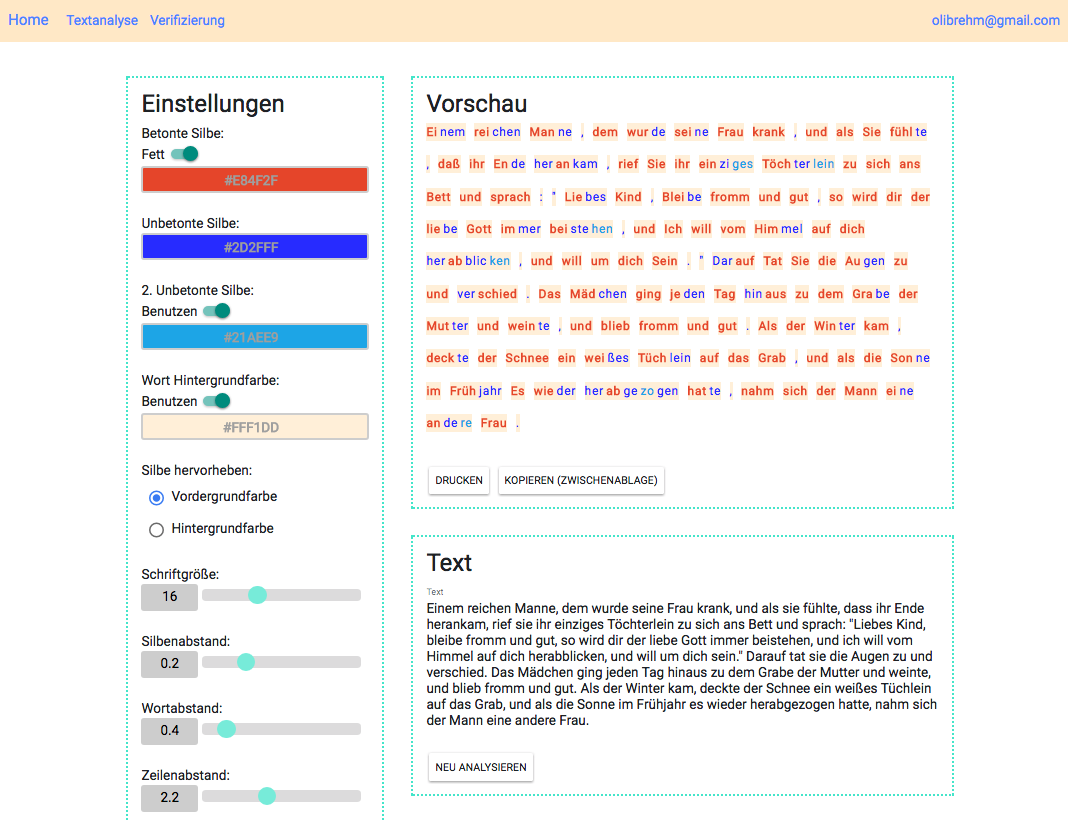
\includegraphics[width=.8\linewidth, frame]{figures/frontend/textanalyse}
	\caption{Bildschirmfoto der Textanalyse}
	\label{fig:frontend-textanalyse}
\end{figure}

\subsubsection{Texteingabe}

Ist noch kein Text analysiert, so zeigt die Text Analyse ein leeres Eingabetextfeld (in Komponente \textit{text\_analysis\_component}). Hier kann ein beliebiger Text eingetippt und analysiert werden.

\begin{figure}[h!]
	\centering
	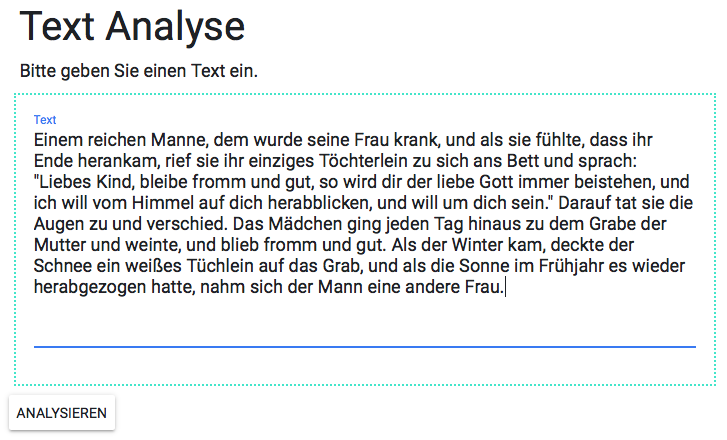
\includegraphics[width=.6\linewidth, frame]{figures/frontend/texteingabe}
	\caption{Bildschirmfoto der Texteingabe}
	\label{fig:frontend-texteingabe}
\end{figure}

\subsubsection{TextAnalysisService}

Der \texttt{TextAnalysisService} wird von mehreren Komponenten verwendet und verwaltet vor Allem eine Instanz der Klasse \texttt{AnnotationText}. Er beinhaltet auch die Logik um einen Eingabetext zu analysieren. Dazu wird ein HTTP Request mit dem Eingabetext an das Backend geschickt. Aus der Antwort kann das Modell des annotierten Texts aufgebaut und in der Vorschau angezeigt werden. Der Service bietet zudem die Funktionen zum Anwenden der aktuellen Annotationseinstellung auf den Text.

\subsubsection{Textvorschau}

Die Textvorschau (Komponente \textit{text\_preview\_component}, gezeigt in Abbildung \ref{fig:frontend-textanalyse}) stellt das Ergebnis der Textannotation so dar, wie es auch im Druck aussehen würde. Die Informationen über die Darstellung (HTML Klassen, CSS Attribute) sind jeweils schon im Datenmodell (in den Wörtern und Silben des \texttt{AnnotationText}) gespeichert und werden im Template der Komponente nur abgerufen. Im Template wird mithilfe von Angular Direktiven über alle Wörter und Silben des Texts iteriert, je nach Typ des Wortes werden verschiedene HTML Tags eingesetzt:
\begin{itemize}
	\item Für jedes annotierte Wort und jede Silbe wird ein \texttt{span} erstellt. Die Klassen und CSS Attribute der  Spans werden mit \textit{Data Binding} (\texttt{[ngClass]} und \texttt{[ngStyle]}, s. Abschnitt \ref{sec:angulardart}) dem Modell entnommen.
	
	\item Für im Text vorkommende Linebreaks (diese werden als \texttt{Word} mit speziellem Typ dargestellt) wird jeweils ein \texttt{<br>} Tag eingesetzt.
	
	\item Für Wörter, welche bei der Analyse nicht in der Datenbank gefunden wurden, wird ein Link (\texttt{span} mit \texttt{(click)} Event) eingesetzt, welcher zur manuellen Wortanalyse (Abschnitt \ref{sec:manuelleanalyse}) führt.
\end{itemize}

Jedes annotierte Wort enthält außerdem eine Subkomponente \texttt{word\_detail\_component}, die beim Klicken auf das Wort als Popup sichtbar gemacht wird. Dieses Popup (Abbildung \ref{fig:frontend-wordconf}) enthält folgende Einstellungen, die für jedes Wort manuell angepasst werden können (eine Änderung hier verändert die grundlegenden Texteinstellungen nicht und hat auch keine Auswirkungen auf die Wortdatenbank oder manuelle Nutzereinträge).

\begin{itemize}
	\item Wort annotieren oder nicht (wird diese Option ausgeschaltet, so wird das Wort ohne Silbentrennung und in der Farbe der unbetonten Silben dargestellt)
	\item Manuelles Betonungsmuster (gilt nur für dieses Wort)
	\item Manuelle Silbentrennung (gilt nur für dieses Wort)
	\item Gleiche Wörter übernehmen (beim Klicken dieses Buttons werden in der Vorschau alle Wörter mit dem gleichen Text genauso annotiert, das ist z.B. bei häufig vorkommenden Eigennamen sinnvoll)
	\item Wortart und Lemma (diese werden nur angezeigt und können nicht verändert werden)
\end{itemize}

\begin{figure}[h!]
	\centering
	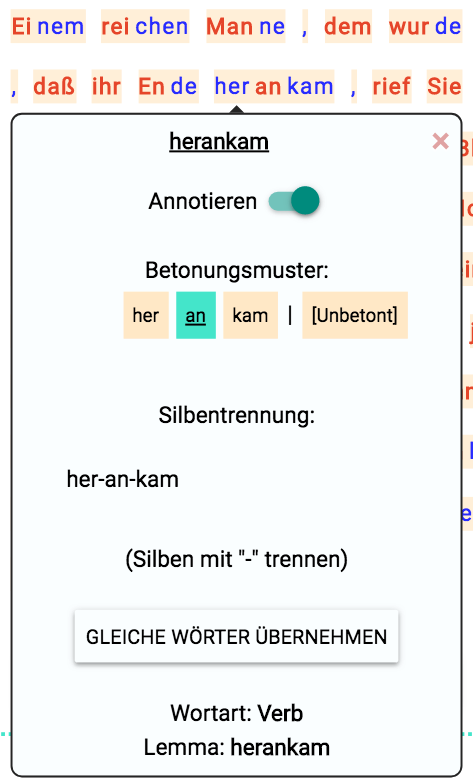
\includegraphics[width=.4\linewidth, frame]{figures/frontend/wordpopup}
	\caption{Bildschirmfoto der spezifischen Worteinstellungen}
	\label{fig:frontend-wordconf}
\end{figure}

Zusätzlich sind im Vorschaufenster Buttons für das Drucken und Kopieren des Texts vorhanden.
\begin{itemize}
	\item Der \textit{Drucken} Button öffnet den Drucken Dialog des verwendeten Browsers. Damit nur der Text in der Vorschau gedruckt wird, wird hier ein eigener CSS Style verwendet. Mit der \texttt{@media print} CSS Anweisung werden dafür alle nicht im Druck benötigten HTML Tags auf \texttt{display: none} gesetzt. und somit ausgeblendet. Zudem wird die Größe des Textvorschau Tags verändert. Ist auf dem Nutzersystem ein PDF Drucker installiert, kann der Text so auch als PDF gespeichert werden.
	
	\item Der Button \textit{Kopieren (Zwischenablage)} kopiert automatisch nur den Vorschautext samt Annotation in die Zwischenablage, sodass dieser z.B. in einem externen Textverarbeitungsprogramm weiter bearbeitet werden kann.
\end{itemize}

\subsubsection{Manuelle Wortanalyse}
\label{sec:manuelleanalyse}

Ist bei der Analyse dem System ein Wort nicht bekannt, so wird es in der Textvorschau rot hinterlegt. Beim Klicken auf das Wort öffnet sich die Manuelle Wortanalyse (Komponente \textit{word\_review\_component}), in der der die Nutzerin oder der Nutzer für dieses Wort das Betonungsmuster und die Silbentrennung selbst bestimmen kann. Hierfür gibt es zum Einen ein Auswahlfenster für die betonte Silbe (durch Klicken kann diese bestimmt werden und wird bei Auswahl in deiner anderen Farbe dargestellt) und zum Anderen ein Textfeld für die Silbentrennung. Hier können manuell Trennstriche gesetzt werden, wobei der Text des Wortes selbst nicht verändert werden darf. Ändert sich bei entsprechender Eingabe die Silbentrennung, passt sich die Eingabe für das Betonungsmuster automatisch an. Mit entsprechenden Buttons kann die Nutzerin oder der Nutzer dann die vorgenommene Analyse entweder speichern, das Wort im Text ignorieren oder ohne zu speichern zum Text zurückkehren.\\

Um die manuellen Eingaben zu erleichtern und zu minimieren werden außerdem automatische Vorschläge generiert. Das Backend sendet für jedes zu bearbeitende Wort eine Liste von Vorschlägen, die aus verschiedenen Quellen stammen können (s. Abschnitt \ref{sec:segmentation-proposals}). Durch Anklicken eines Vorschlags wird dieser in den Eingabefenstern auf der linken Seite übernommen.

\todo{irgendwo muss noch segmentation service und segmentation proposal service rein}

\begin{figure}[h!]
	\centering
	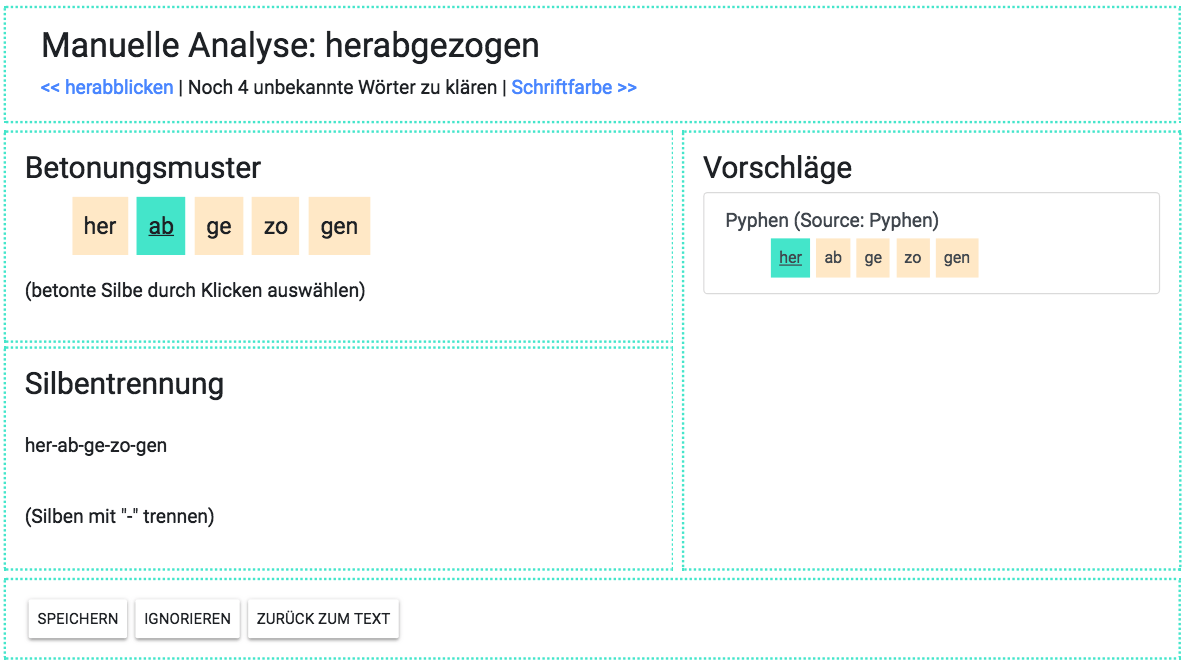
\includegraphics[width=.8\linewidth]{figures/frontend/manuelle-analyse}
	\caption{Bildschirmfoto der Manuellen Wortanalyse\todo{bild wo MARY funktioniert!}}
	\label{fig:frontend-manuelle-analyse}
\end{figure}

\subsubsection{Textoptionen}

Unter dem Textvorschaufenster befinden sich weitere Fenster zur Verwaltung des aktuellen Texts (Komponente \texttt{text\_input\_component}). Folgende Funktionen (in drei Kästen, von oben nach unten) werden hier noch angeboten:
\begin{itemize}
	\item Der aktuelle Text wird in einem Eingabefeld angezeigt. Dieser kann hier verändert und neu analysiert werden.
	\item Der aktuelle Text kann im Nutzerkonto (s. Abschnitt \ref{sec:nutzerkonto}) gespeichert werden. Dazu muss ein Titel eingegeben werden. Wird anschließend der \textit{Speichern} Button gedrückt, wird der Text mit zugehörigem Titel vom \texttt{UserAccountService} gespeichert.
	\item Die aktuelle Analyse kann vollständig verworfen werden, sodass wieder das ursprüngliche, leere Textfeld angezeigt wird.
\end{itemize}

\subsection{Annotationseinstellungen}

Im Kasten links neben der Textvorschau können die Einstellungen verändert werden, die die Art der Annotation bestimmen. Die Einstellungen werden zentral in einem Objekt der Klasse \texttt{TextConfiguration} im \texttt{TextAnalysisService} gespeichert und nach Nutzereingaben auf den aktuellen Text angewandt. Wird hier eine Farbe oder ein Abstand verändert, so ist dies sofort in der Textvorschau sichtbar. Außerdem kann die aktuelle Konfiguration jederzeit als Vorlage gespeichert werden, so kann sie später (z.B. für einen anderen Text) wiederverwendet werden. Das User Interface für die Einstellungen ist in der Komponente \texttt{text\_settings\_component} definiert.

\subsubsection{User Interfache für Einstellungen}

Ganz oben können zunächst Farben für die Annotation und die Art, wie diese verwendet werden eingestellt werden (Abbildung \ref{fig:frontend-colorconf}):

\begin{itemize}
	\item \textit{Betonte Silbe}: Hier wird die Farbe für die betonte Silbe in jedem Wort festgelegt. Außerdem kann gewählt werden, ob der Text der Silbe fett dargestellt werden soll. Für die Auswahl der Farben wurde ein entsprechend farbiger Kasten verwendet, der beim Anklicken den Farbwahldialog des Browsers öffnet.
	
	\item \textit{Unbetonte Silbe}: Alle unbetonten Silben werden in dieser Farbe dargestellt.
	
	\item \textit{2. Unbetonte Silbe}: In längeren Wörtern folgen mehrere unbetonte Silben aufeinander. Wird diese Option aktiviert, werden aufeinanderfolgende unbetonte Silben abwechselnd in den Farben der 1. und der 2. unbetonten Silbe dargestellt.
	
	\item \textit{Worthintergrundfarbe}: Ist diese Option aktiviert erhält zusätzlich jedes Wort (über Silbengrenzen hinaus) eine Hintergrundfarbe. Dies ist z.B. dann sinnvoll, wenn man große Abstände zwischen den einzelnen Silben wählt, so kann das Wort trotzdem als Einheit erfasst werden.
	
	\item \textit{Silbe hervorheben}: Hier kann gewählt werden, ob die Silbenfarben als Schriftfarbe (\textit{Vordergrundfarbe}) oder Hintergrundfarbe benutzt werden
\end{itemize}

Beispiele zu verschiedenen Einstellungen sind in der Evaluation in Abschnitt \ref{sec:annotation-results} zu finden.

\begin{figure}[h!]
	\centering
	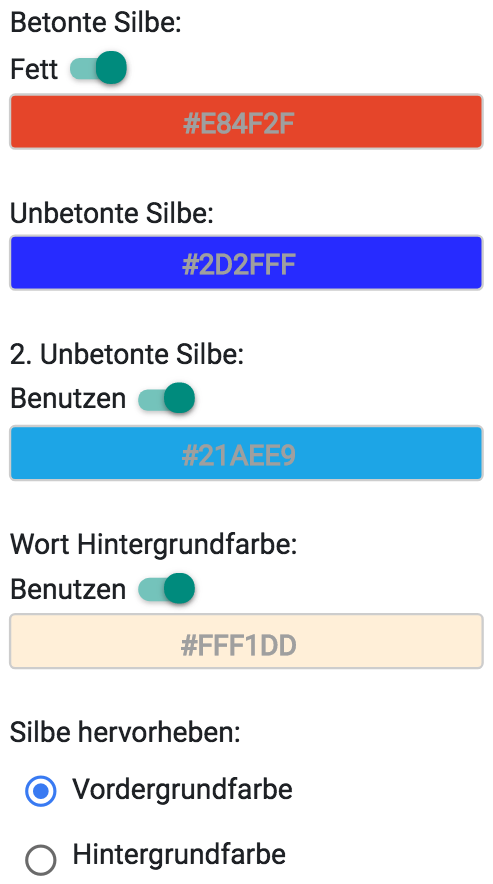
\includegraphics[width=.4\linewidth, frame]{figures/frontend/config-color}
	\caption{Bildschirmfoto der Farbeinstellungen}
	\label{fig:frontend-colorconf}
\end{figure}

Unter den Farbeinstellungen lassen sich verschiedene Größen und Abstände im Text definieren (Abbildung \ref{fig:frontend-textconf}):
\begin{itemize}
	\item Schriftgröße
	\item Silbenabstand (Abstand zwischen einzelnen Silben)
	\item Wortabstand (Abstand zwischen ganzen Wörtern)
	\item Zeilenabstand
	\item Zeichenabstand (Abstand zwischen den einzelnen Buchstaben eines Wortes)
\end{itemize}

\begin{figure}[h!]
	\centering
	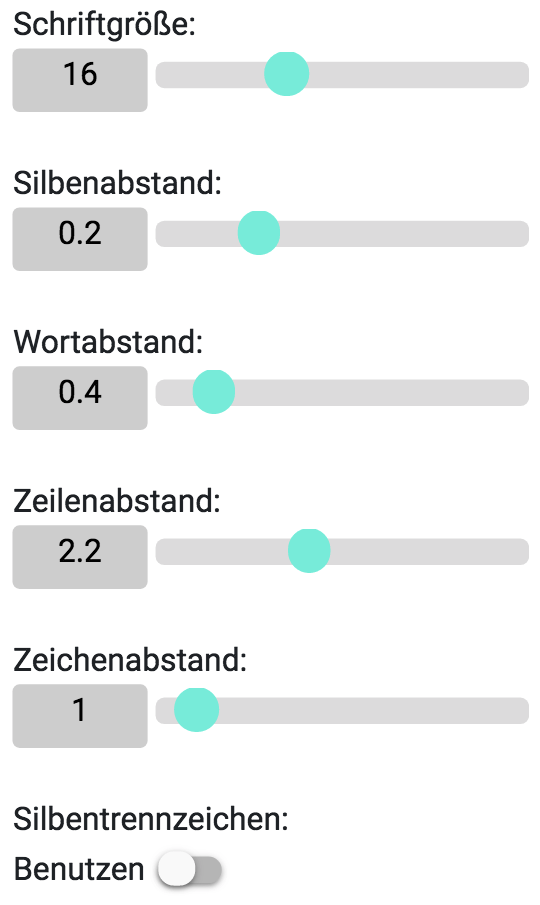
\includegraphics[width=.4\linewidth, frame]{figures/frontend/config-text}
	\caption{Bildschirmfoto der Texteinstellungen}
	\label{fig:frontend-textconf}
\end{figure}

Alle Werte lassen sich hier mithilfe eines Sliders einstellen. Außerdem gibt es die Möglichkeit, ein beliebiges Zeichen als Silbentrennzeichen zu benutzen, was dann im Zwischenraum zwischen allen Silben im Text erscheint.\\

An letzter Stelle in den Einstellungen steht ein Dropdown Menü, in dem man eine Wortart auswählen kann (Abbildung \ref{fig:frontend-pos-einstellungen}). Für jede Wortart lassen sich folgende Einstellungen vornehmen, die dann auf den gesamten Text angewandt werden:
\begin{itemize}
	\item \textbf{Annotieren}: Aktiviert die Annotation für Wörter dieser Wortart, d.h. Silben werden getrennt und in den gewählten Farben dargestellt).
	
	\item \textbf{Unbetont}: Die Annotation ist zwar aktiv und Silben werden getrennt dargestellt, allerdings wird die betonte Silbe nicht besonders hervorgehoben.
	
	\item \textbf{Ignorieren}: Das Wort wird ohne Trennung von Silben in der Farbe der unbetonten Silbe dargestellt.
\end{itemize}

Ändert die Nutzerin oder der Nutzer eine Einstellung, so wird im \texttt{AnnotationText} über sämtliche Wörter iteriert und deren Einstellung entsprechend angepasst.

\begin{figure}[h!]
	\centering
	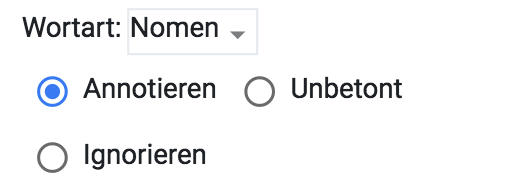
\includegraphics[width=.4\linewidth, frame]{figures/frontend/config-pos}
	\caption{Bildschirmfoto der spezifischen Wortart Einstellungen}
	\label{fig:frontend-pos-einstellungen}
\end{figure}

\subsubsection{Annotationsvorlagen}

Im Kasten unterhalb der Annotationseinstellungen können Konfigurationen verwaltet werden. Jedem Nutzerkonto sind Vorlagen zugeordnet, d.h. jede Nutzerin und jeder Nutzer verwaltet und sieht nur ihre oder seine eigenen Vorlagen. In der Vorlage werden sämtliche Einstellungen gespeichert, das ganze \texttt{TextConfiguration} Objekt wird hier an das Backend geschickt und serialisiert.\\

Sind bereits Vorlagen vorhanden, werden diese hier aufgelistet. Sie können ausgewählt (und damit auf den aktuellen Text angewandt) werden oder durch Klicken auf das kleine \textit{X} rechts neben dem Vorlagennamen gelöscht werden. Darunter befindet sich ein Textfeld für den Namen einer neu anzulegenden Vorlagen. Beim Klicken des \textit{Vorlage speichern} Buttons wird diese dann unter dem gewählten Namen (und mit den momentan aktiven Einstellungen) neu gespeichert oder, wenn die Vorlage schon existiert überschrieben.

\begin{figure}[h!]
	\centering
	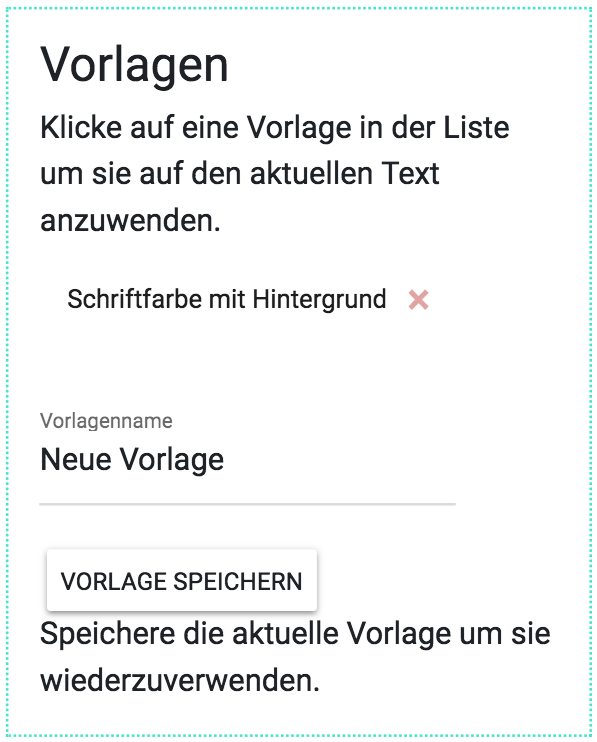
\includegraphics[width=.4\linewidth]{figures/frontend/config-vorlagen}
	\caption{Bildschirmfoto der UI zur Verwaltung und Verwendung von Annotationsvorlagen}
	\label{fig:frontend-vorlagen}
\end{figure}

\subsection{Nutzerkonto}
\label{sec:nutzerkonto}

Die Nutzerkonto Seite zeigt entweder das Formular zum Einloggen oder Konto erstellen an, oder falls die Nutzerin oder der Nutzer schon eingeloggt ist, Informationen und Inhalte des Nutzerkontos. Die Komponente \texttt{user\_account\_component} lagert einige Funktionalitäten wie die Registrierung oder die Liste von Nutzertexten in Subkomponenten aus.

\subsubsection{UserAccountService}

Der \texttt{UserAccountService} speichert die Informationen zum aktiven Nutzerkonto, z.B. Email Adresse und Passwort, sowie eine Liste von Nutzertexten und manuell segmentierten Wörtern. Er bildet alle Funktionen ab (z.B. Anglegen, Auflisten oder Löschen), die zum Verwalten von Nutzerkonten, Nutzertexten und Wörtern notwendig sind. Dafür werden jeweils HTTP Requests an das Backend gesendet und die erhaltenen Antworten weiter verarbeitet.

\subsubsection{Login und Registrierung}

Ist kein Nutzer eingeloggt, so wird zuerst das Login Formular angezeigt. Außerdem lautet der Link rechts oben in der Navigationsleiste \textit{Login}, sodass der Login schnell gefunden werden kann. Loggt sich eine Nutzerin oder ein Nutzer mit einem bereits bestehenden Konto ein, so enthält der Navigationslink die Email Adresse des Nutzerkontos.\\

Unter dem Login Formular führt ein Link mit der Aufschrift \textit{Neues Konto erstellen} auf die Registrierungsseite. Hier muss für die erfolgreiche Registrierung eine Email Adresse sowie ein Passwort eingegeben werden. Außerdem speichert das Nutzerkonto Vor- und Nachname, sowie die Information, ob es sich bei dem neu anzulegenden Konto um ein Expertenkonto handelt, was in einer Checkbox angegeben werden kann. Expertenkontos sollen von SprachtherapeutInnen oder NachhilfelehrerInnen genutzt werden.  Diese verfügen bei der Verifizierung über eine schwerer gewichtete Stimmt (s. Abschnitt \ref{sec:verification-service}). Wird die Registrierung abgeschickt wird das neue Nutzerkonto im Backend erstellt und die Nutzerkontoseite kehrt zum Login Formular zurück. Schlägt das Registrieren fehl (z.B wenn es schon ein Konto mit der eingegebenen Email Adresse gibt, oder weil Eingaben fehlen) wird eine entsprechende Fehlermeldung angezeigt.

\subsubsection{Nutzerkonto Seite}

Ist aktuell eine Nutzerin oder ein Nutzer eingeloggt, werden Informationen zum Konto, sowie Listen von gespeicherten Texten und manuell segmentierten Wörtern angezeigt.\\

Die Liste der gespeicherten Nutzertexte zeigt zunächst nur deren Titel als Links an (Komponente \texttt{user\_textlist\_component}). Werden diese angeklickt, sieht man den Text und hat die Möglichkeit, diesen für die Analyse zu verwenden oder zu löschen. Klickt man auf den Button \textit{Verwenden}, wechselt die Applikation zur Textanalyse und analysiert den gewählten Text. \\

Unter der Textliste ist die Liste manuell segmentierter Wörter zu finden (Komponente \texttt{user\_wordlist\_component}). Die Einträge zeigen den Worttext, die Silbentrennung und das Betonungsmuster der Segmentierung. Die Einträge können auch gelöscht werden, z.B. falls ein Fehler bei deren Erstellung unterlaufen ist.\\

Ganz unten auf der Seite sind Buttons zum Ausloggen und Löschen des Kontos vorhanden.

\begin{figure}[h!]
	\centering
	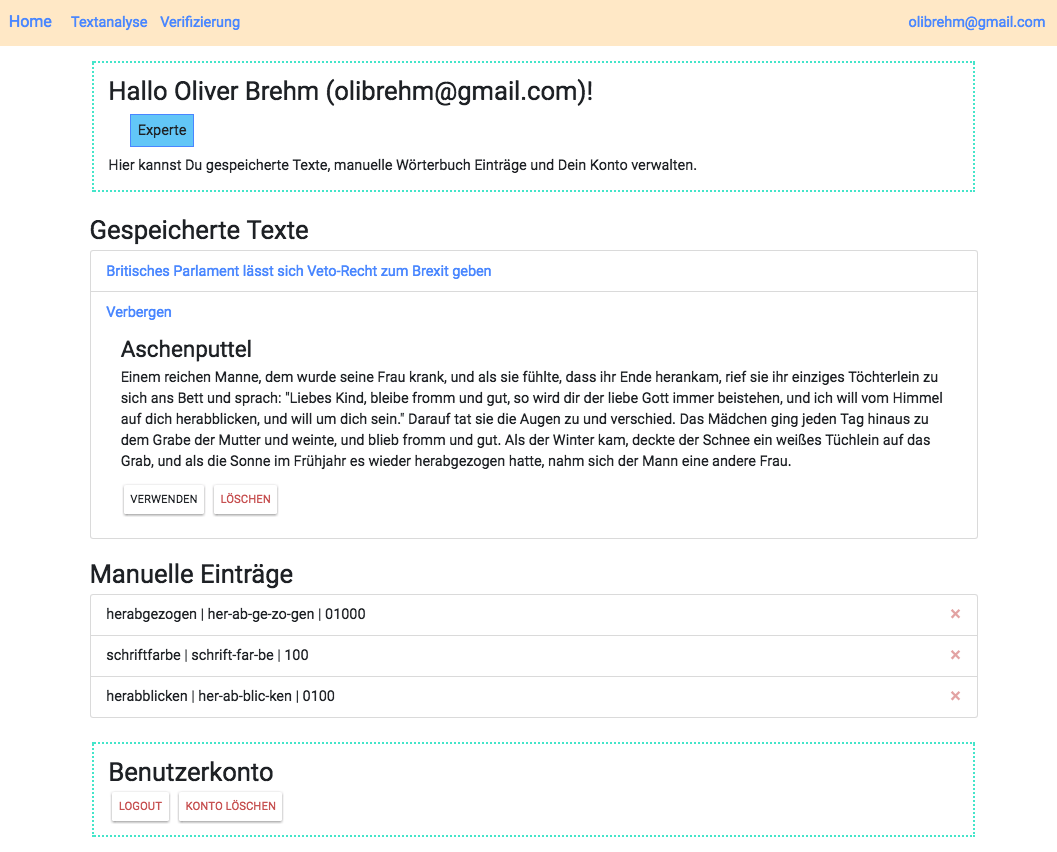
\includegraphics[width=.8\linewidth, frame]{figures/frontend/user-account}
	\caption{Bildschirmfoto der Nutzerkontoseite}
	\label{fig:frontend-useraccount}
\end{figure}

\subsection{Wort-Verifizierung}

Die Wort Verifizierung dient der Bestätigung von manuellen Segmentierung von NutzerInnen durch andere NutzerInnen, sodass diese in die globale Wortdatenbank aufgenommen werden können (s. Abschnitt \ref{sec:verification-service}). Das User Interface für diesen Prozess ist in der Komponente \texttt{word\_verification\_component} implementiert.\\

Ist eine Nutzerin oder ein Nutzer eingeloggt, werden nacheinander zu verifizierende Wörter geladen, das User Interface ähnelt dem, das zur manuellen Analyse von unbekannten Wörtern verwendet wird (s. Abschnitt \ref{sec:manuelleanalyse}). Auch hier gibt es jeweils eine Eingabemöglichkeit zur Auswahl der betonten Silbe und zur Bestimmung der Silbentrennung. Auf der Rechten Seite befinden sich allerdings neben den automatisch generierten Vorschlägen auch die Segmentierungsvorschläge anderer NutzerInnen. Automatisch wird der Vorschlag der Nutzerin oder des Nutzers ausgewählt, die die Segmentierung zuerst erstellt hat. Haben weitere NutzerInnen den Vorschlag schon verifiziert, so erscheinen auch deren Segmentierungen in der Liste. \\

Zur eigentlichen Verifizierung kann nun ein Eintrag in der Liste der Vorschläge ausgewählt werden oder, falls alle Vorschläge als falsch empfunden werden, ein andere Segmentierung auf der linken Seite eingestellt werden. Danach wird die Verifizierung mit dem Button \textit{Abschicken} gespeichert.\\
Sind noch weitere zu verifizierende Einträge vorhanden, wird sofort das nächste Wort geladen. Ein Label unter der Überschrift der Komponente zeigt an, wie viele zu verifizierende Wörter es noch gibt.

\begin{figure}[h!]
	\centering
	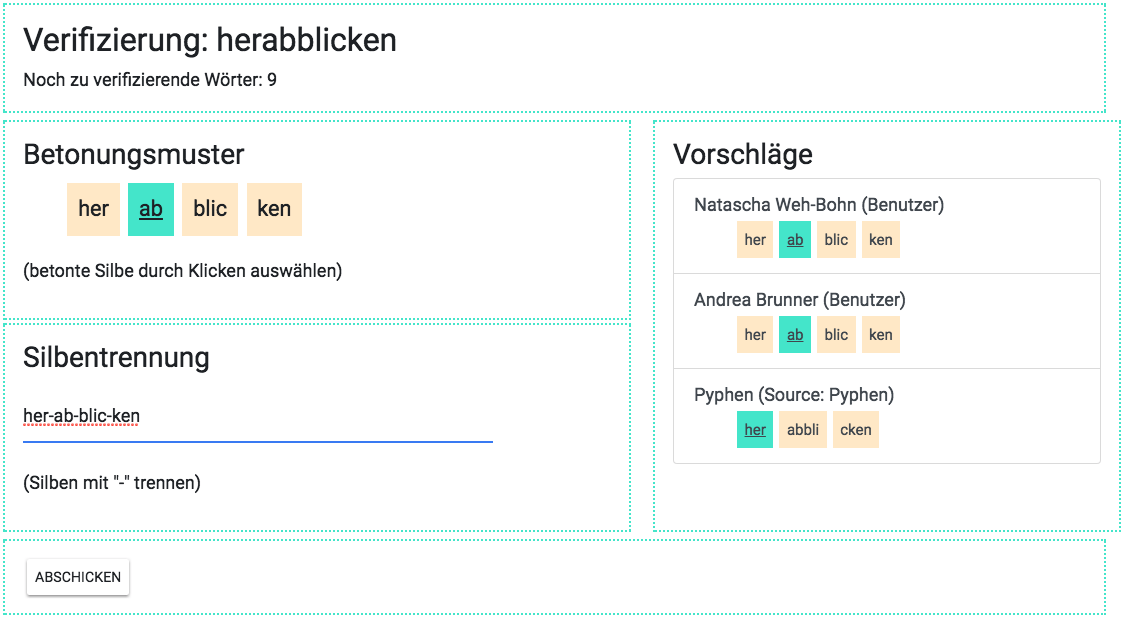
\includegraphics[width=.8\linewidth]{figures/frontend/verifizierung}
	\caption{Bildschirmfoto der Verifikation von manuell hinzugefügten Wörtern}
	\label{fig:frontend-verification}
\end{figure}